\documentclass[tikz,border=5pt]{standalone}
\usepackage{amsmath}
\usetikzlibrary{arrows.meta,positioning,fit,calc}

\begin{document}
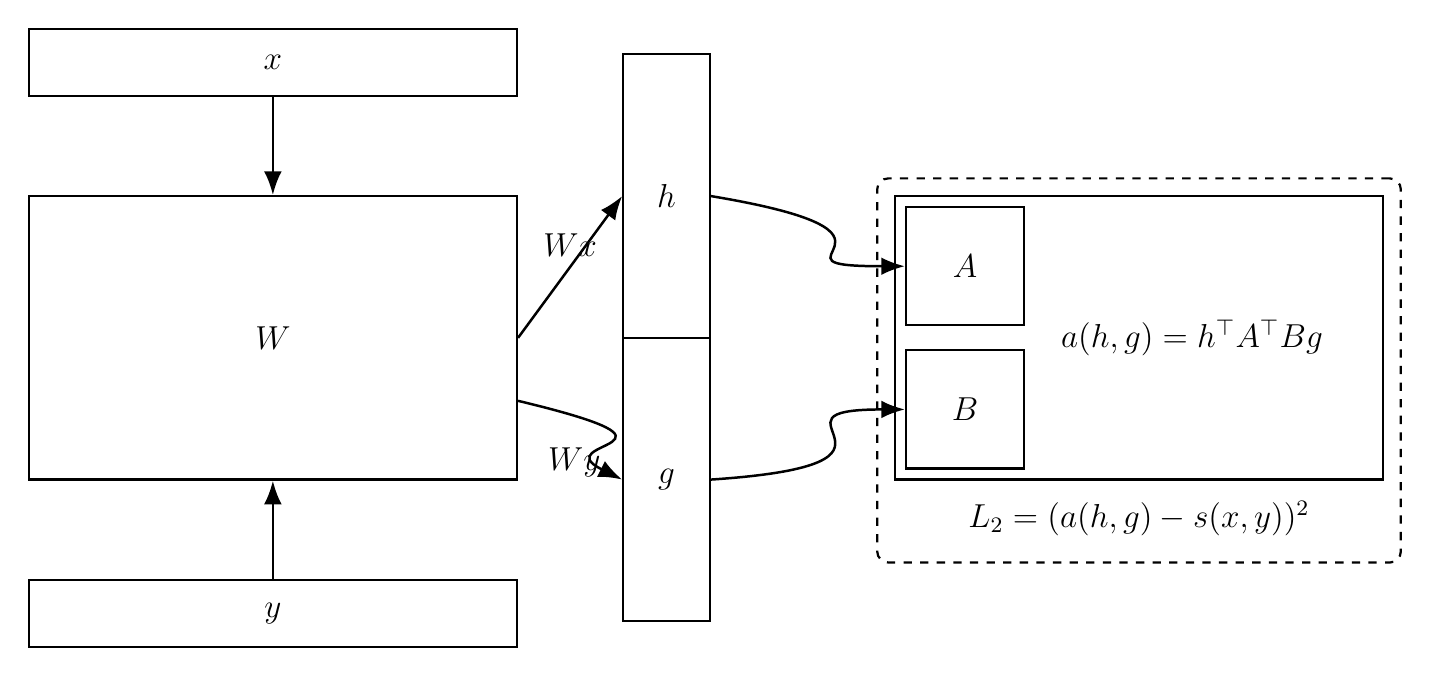
\begin{tikzpicture}[font=\large,node distance=3.5cm]
  %----- styles
  \tikzset{
    box/.style   ={draw,thick,minimum width=6.2cm,minimum height=3.6cm,align=center},
    slim/.style  ={draw,thick,minimum width=1.1cm,minimum height=3.6cm,align=center},
    var/.style   ={draw,thick,minimum width=6.2cm,minimum height=0.85cm},
    arrow/.style ={-{Latex[length=3mm]},line width=0.9pt},
    dashedbox/.style ={draw,dashed,rounded corners,inner sep=6pt,thick},
    smallsq/.style={draw,thick,minimum width=1.5cm,minimum height=1.5cm}
  }

  %==================== COLUMN LAYOUT ====================
  % Column X positions for clear spacing
  \def\xW{0}     % W column
  \def\xHG{5}    % h/g column (middle)
  \def\xA{11}    % a(h,g) column (right)

  %----- nodes
  % Left column: W with x/y
  \node[box] (W) at (\xW,0) {$W$};
  \node[var] (x) at (\xW, 3.5) {$x$};
  \node[var] (y) at (\xW,-3.5) {$y$};

  % Middle column: h (up) and g (down)
  \node[slim] (h) at (\xHG, 1.8) {$h$};
  \node[slim] (g) at (\xHG,-1.8) {$g$};

  % Right column: a(h,g) module centered, with A/B inside and L2 below
  \node[box,align=left] (ybox) at (\xA,0) {};
  \node[anchor=west] at ($(ybox.west)+(2.0,0)$) {$a(h,g) = h^\top A^\top B g$};
  \node[smallsq,anchor=north west] (sq1) at ([xshift=4pt,yshift=-4pt]ybox.north west) {$A$};
  \node[smallsq,anchor=south west] (sq2) at ([xshift=4pt,yshift=4pt]ybox.south west) {$B$};
  \node (L2) [below=4pt of ybox] {$L_2 = (a(h,g) - s(x,y))^2$};
  \node[dashedbox,fit=(ybox)(L2)] {};

  %----- connections
  % x -> W, y -> W
  \draw[arrow] (x.south) -- (W.north);
  \draw[arrow] (y.north) -- (W.south);

  % W -> h (top path)
  \draw[arrow] (W.east) -- node[above] {$Wx$} (h.west);

  % W -> g (bottom path; gentle curve)
  \coordinate (Wexit) at ($(W.east)+(0,-0.8)$);
  \draw[arrow] (Wexit) .. controls +({(\xHG-\xW)/2},-0.6) and +(-1,0.5) .. (g.west)
    node[anchor=east, pos=0.45, xshift=-2pt, yshift=-8pt] {$Wy$};

  % h -> A (curved, aligned toward A midpoint)
  \draw[arrow] (h.east) .. controls +({(\xA-\xHG)/2},-0.5) and +(-2,0.0) .. (sq1.west);

  % g -> B (curved, aligned toward B midpoint)
  \draw[arrow] (g.east) .. controls +({(\xA-\xHG)/2},0.2) and +(-2,0.0) .. (sq2.west);

\end{tikzpicture}
\end{document}
